\documentclass{article}

\usepackage{multicol}
\usepackage{lipsum}
\usepackage{graphicx}
\graphicspath{{images/}}
\usepackage{blindtext}
\usepackage{subfiles} % Best loaded last in the preamble
\usepackage[dvipsnames]{xcolor}
\usepackage[T1]{fontenc}
\usepackage{setspace}
\usepackage{float}
\usepackage{array}

\setlength{\columnsep}{1cm}

\usepackage{fullpage, tikz}
\usepackage{eso-pic}
\AddToShipoutPictureBG{%
	\begin{tikzpicture}[remember picture, overlay]
		\node[opacity=.4, inner sep=0pt]
		at(current page.center){
\includegraphics[width=8.5in, height=11in]{images/background}};
	\end{tikzpicture}%
}

\usepackage[margin={1.5cm,1.5cm}]{geometry}

\newcommand\BackgroundPic{%
	\put(0,0){%
		\parbox[b][\paperheight]{\paperwidth}{%
			\vfill
			\centering
			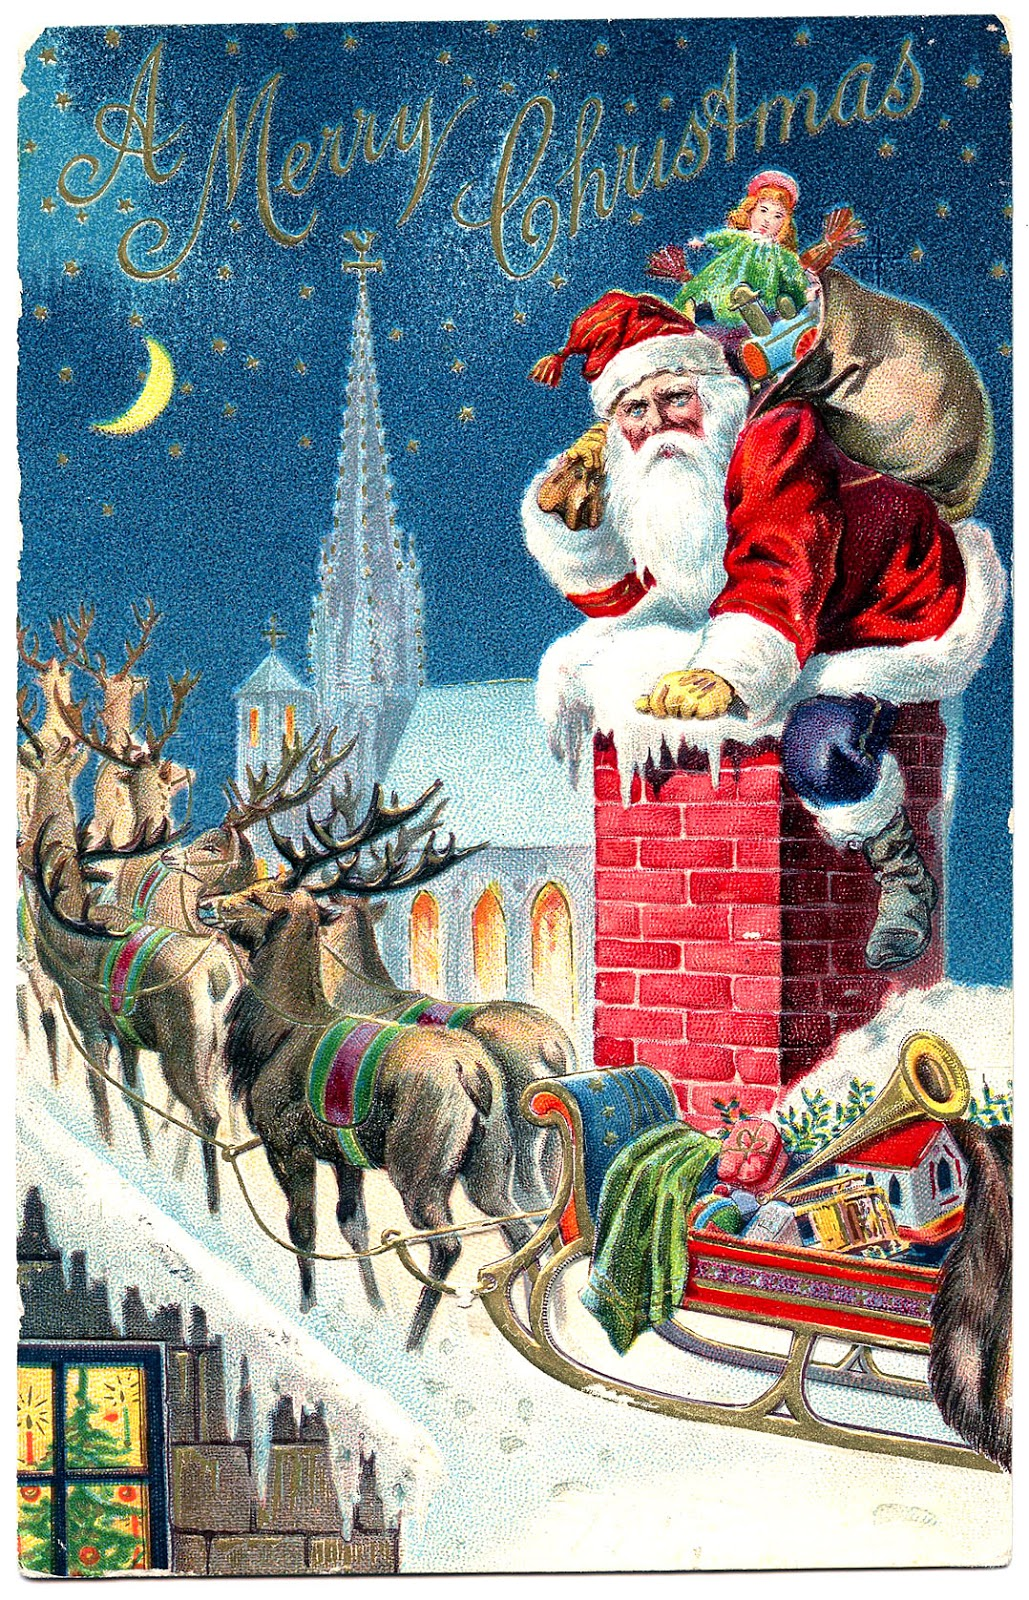
\includegraphics[width=\paperwidth,height=\paperheight]{images/cover.jpg}%
			\vfill
}}}

\title{\color{white}\textsc{\Huge Winter Solstice Sabotage }}
\date{ }


\setlength\fboxsep{8pt}

\begin{document}
	\AddToShipoutPicture*{\BackgroundPic}
	\maketitle
	\pagebreak
	\begin{multicols*}{2}
	\section{Introduction}
	
	\subsection*{Overview}
	The \emph{Winter Solstice Sabotage} one-off adventures is meant to be played with a group of 5 players at level 4. The adventure is meant to be completed in one session.
	
	It is a Christmas inspired story with familiar themes and characters. The plot of the story revolves around the character \emph{Klauss Atnas} (Santa Claus) whom has lost his powers to an evil gnome named \emph{Mister Frink}. The adventurers must help \emph{Klauss} find the evil gnome and defeat him to lift the curse and restore the blessing of the winter solstice.
	
	\subsection*{Adventure Hook}
	After a long year of adventures and treasure hunting, the adventurers find themselves returning home to celebrate the winter solstice when they are caught in a massive blizzard. They are forced to stop and find shelter, and happen to come across a tavern called the \emph{The Jolly Reindeer}. They enjoy a quiet meal with other guests lost in the storm when suddenly they hear a loud thump on which appears to come from the roof. Terrified, the hosts and other patrons try to convince the adventurers to go investigate what caused the loud noise on the roof.
	
	Upon investigating they find Klauss Atnas (Santa Claus) kneeling down below a large slay pulled by strange creatures with large antlers. Klauss is an other white bearded gnome wearing a Santa style robe and hat. Klauss appears to be attempting to fix the giant slay when he is startled by the adventurers. In a panic he attempts to activate his invisibility necklace but is unaware that the necklace's power has faded and is not concealing him. Once he realizes that the players can see and hear him, he explains who he is and how he brings blessings to each home in the world during the winter solstice festival. When he realizes that his powers have gone, he tries to recruit the adventurers to help him solve this mystery. The assumption here is the players will agree to this to move the story along, otherwise Klauss will simply kidnap them.
	
	Due to the emergency, Klauss uses an emergency magical device which transports him and all the players to what is suppose to be Northerland (north pole). Unfortunately the device malfunctions and they find themselves outside the Northerlands in a snowy plains in the middle of blizzards. Confused, it takes Klauss a moment to comprehend the malfunction and realize where they are located. He looks at his compass it is completely indicating the wrong direction. After some time he finally is able to determine his location and remembers an ancient cave used in the past for tracking winter solstice operations. 
	
	\section{The Abandoned Cavern}
	
	Klauss leads the players to an abandoned cave which once acted as a base of operations for the winter solstice festival blessing. The entrance of the cave is dark and there appears to be a large locked metal door. Klauss tries to remember the password but can't remember exactly (get creative with password ideas). He finally gets the right password (two turtledoves and a partridge in a pear tree). The door opens and torches light to illuminate a large cavern. Klauss rushes to the other side of the cavern where a console with various controls is located.
	
	Klauss fails to notice a hidden \emph{Snow Owlbear} hidden in the snow around the cavern. Unless the players proceed carefully by using perception, investigation or stealth, the \emph{Snow Owlbear} surprises the adventurers (run the owlbear encounter). Klauss will join the fight although we is generally not a fighter, he mainly focuses on using his protective and defensive abilities to help the adventurers.
	
	Once the owlbear is defeated, it drops a lump of coal with a strange symbol on it. Klauss immediately recognizes it as \emph{Mr. Frink}'s calling card. To his dismay, it appears \emph{Mr. Frink} has somehow infiltrated the Northerland village and has corrupted it's magical powers. Klauss asks the players to travel to Northerland village and attempt to find and apprehend Mr. Frink before the winter solstice festival is over. He hands the players a working compass which will lead them to the Northerland village. In addition, he gives them the defective device which contains the corrupted device and asks the adventurers if they can get help from the other gnomes to discover why it's been corrupted.
	
	\colorbox{GreenYellow}{\begin{minipage}{0.4\textwidth}
		Players who investigate the corrupted device learn that it's compass actually points in the exact opposite direction as the functioning device. In fact, the adventurers should learn later that Mr. Frink's presence repels the compass' needle. The players can use this to determine which of the gnomes is in fact \emph{Frink}. 			
	\end{minipage}}
	\break
	
	Klauss must continue his blessing delivery if he is to complete it before the end of the winter solstice. He manages to tap enough magical energy from the console to power his slay and reindeer to continue his journey. Before he leaves them, he gives them custody of Durolph the red nosed reindeer to ride to the Northerland village. Durolph grows large enough to accommodate all the adventurers to ride it. He also urges the adventurers to hurry because Mr. Frink's power grows every passing moment. 
	
	\section{Northerland Village}

	The adventurers travel on Durolph's back through the snow planes and blizzard towards Northerland village. After about an hour of travel, they finally arrive at a lone small log cabin covered in snow. The gnome clerk at the desk doesn't appear to be paying attention to the players. Once the clerk realizes that the adventurers are not the regular visitors he is accustomed to, he is surprised and nervous. The players will have to persuade him the let them into the village, with advantage if they show him Klauss' devices. The clerk doesn't know much about Mr. Frink and finds the idea of him infiltrating Northerland village laughable.
	
	Once persuaded, the clerk let's the players through a back door which opens to another world. Northerland village is a bustling town full of gnomes who are especially busy during the winter solstice celebration. The village contains many homes and a huge factory where gnomes are working on building statues and idols used in the blessings. The village is protected by a giant magical bubble shield. There are thousands of gnomes running around, so finding the impostor Mr. Frink will be like trying to find a needle in a haystack. Most of the gnomes are so busy they just completely ignore the players.
	
	At this point, you should start some sort of timer or keep track of the players actions to determine how much time has passed. Mr. Frink starts with a power level of 3 (increase to 4 or 5 to increase the difficulty). You can periodically increase his power at your discretion if the players are taking to long or are failing to progress towards finding him. Keep track of his power level as it will determine how many clones and how strong Mr. Frink will be. Each time the power level increases, a power drain occurs momentarily, causing lights to dim. This will be used as a sign to the players to hurry their search for Mr. Frink.
	
	The easiest way to find Mr. Frink is to use the corrupted compass. The closer the compass is to Frink, the more the needle will vibrate. The needle will always point away from him, so it can be used as a guide. The players might be savvy enough to determine this without extra clues, but if not, they will need to investigate around town to find more clues.
	
	\subsubsection*{\underline{3. Northerland Administration Office}}
	
	In the center of the town is a the main administration building where players can find extra clues to help in their investigation in finding Frink. The head administrator gnome named \emph{Frosty} can provide some information for the players. He is more inclined to take the Mr. Frink threat seriously. He is aware of the basic history and legends surrounding him but will need to check the archives.
	
	If the players choose to try to find clues in the archives, add a level of power to Mr. Frink. In the archives, the players can use any intelligence skill they desire to search the archive records. Based on the skill type and roll, players can discover clues about Mr. Frink. Refer to the tables below to determine which clues to reveal based on the skills. If any of the clues regarding mistletoe are discovered, Frosty gives the adventurers bundles of mistletoe to help them.
	
	\begin{table}[H]
		\begin{tabular}{|m{2.5em}|m{20em}|}
			\hline
			\textbf{d20} & \textbf{Arcana Roll Results} \\
			\hline
			\hline
			1-4 & Failure, add +1 power level to Mr. Frink. \\
			\hline
			5-8 & No clue  \\
			\hline
			9-12 & Mr Frink is vulnerable to fire. \\
			\hline
			13-15 & Mr. Frink is a master of disguise and it is said that he can even magically replicate himself. \\ 
			\hline
			16-18 &  Destroying his clones will reveal his true identity. \\
			\hline
			19+ & Mr. Frink's clones can be destroyed by solving riddles or by attacking the real him. Hurting a clone or failing to answer the riddle will freeze the target. \\
			\hline
		\end{tabular}
	\end{table}

	\begin{table}[H]
		\begin{tabular}{|m{2.5em}|m{20em}|}
			\hline
			\textbf{d20} & \textbf{History Roll Results} \\
			\hline
			\hline
			1-4 & Failure, add +1 power level to Mr. Frink. \\
			\hline
			5-8 & No clue  \\
			\hline
			9-12 & Mr Frink is as old if not possibly older than Klauss. \\
			\hline
			13-15 & Mr. Frink is from the Southerlands, the southern most known location in the world. \\ 
			\hline
			16-18 & Mr. Frink has successfully infiltrated Northerland village about two millennia ago, but was caught and banished. \\
			\hline
			19+ & Mr. Frink historically repeats the same riddles, most of which relate to the winter solstice. The riddles themselves were not recorded but some of the answers have been. The answers to some of the riddles include: a snowflake, a candle, a snowman, a wreath, and mistletoe. Last time he infiltrated, he was successfully defeated by correctly answering his riddles. \\
			\hline
		\end{tabular}
	\end{table}

	\begin{table}[H]
		\begin{tabular}{|m{2.5em}|m{20em}|}
			\hline
			\textbf{d20} & \textbf{Investigation Roll Results} \\
			\hline
			\hline
			1-4 & Failure, add +1 power level to Mr. Frink. \\
			\hline
			5-8 & No clue \\
			\hline
			9-12 & Mr Frink siphons energy from Northerland village causing power outages. \\
			\hline
			13-15 & Mr. Frink's power grows gradually the longer is in Northerland village during the winter solstice \\ 
			\hline
			16-18 &  Mr. Frink's presence affect the magnetic fields around Northerland village. \\
			\hline
			19+ & Finding him could be accomplished by reversing the polarity on a regular compass, which will cause the needles to point directly to his location. \\
			\hline
		\end{tabular}
	\end{table}

	\begin{table}[H]
		\begin{tabular}{|m{2.5em}|m{20em}|}
			\hline
			\textbf{d20} & \textbf{Nature Roll Results} \\
			\hline
			\hline
			1-4 & Failure, add +1 power level to Mr. Frink. \\
			\hline
			5-8 & No clue  \\
			\hline
			9-12 & Mr Frink is not a gnome, he's some entirely different creature. Although it is possible that at some point he was, and was simply corrupted. \\
			\hline
			13-15 & Mr. Frink is does not have dark-vision, therefore he struggles to see in the dark. \\ 
			\hline
			16-18 &  Mr. Frink's emits some sort of powerful magnetic energy field.  \\
			\hline
			19+ & Mr. Frink's is reportedly extremely allergic to mistletoe and could be useful for warding him off. \\
			\hline
		\end{tabular}
	\end{table}

	\begin{table}[H]
		\begin{tabular}{|m{2.5em}|m{20em}|}
			\hline
			\textbf{d20} & \textbf{Religion Roll Results} \\
			\hline
			\hline
			1-4 & Failure, add +1 power level to Mr. Frink. \\
			\hline
			5-8 & No clue  \\
			\hline
			9-12 & Mr Frink is evil and hates all good blessings. \\
			\hline
			13-15 & Mr Frink believes he is a divine entity and wants to rule over Northerland. \\ 
			\hline
			16-18 & Mr. Frink likes to disguise himself and conceal himself in plain sight in a very busy area. \\
			\hline
			19+ & A legend speaks of a way to defeat Mr. Frink for good by giving him a kiss under a mistletoe.\\
			\hline
		\end{tabular}
	\end{table}

	
	
	\section{Mr. Frink}
	
	At this point, the players should have enough clues to find Mr. Frink. Frink is located in the main factory hiding among all the gnomes working. The factory is huge and there are thousands of gnomes running around fabricating idols and statues for the winter solstice blessing. Most are too busy to talk or interact with the adventurers. The easiest and quickest way to find Mr. Frink is using the defective compass which vibrates more as the players approach him. 
	
	If the players use other methods, add a power level to Mr. Frink accordingly. Other methods used to find him might be turning off the lights, or using mistletoe, or possibly other creative solutions. Eventually, the adventurers should be able to discover which of the gnomes is Mr. Frink in disguise. Once discovered, Mr. Frink attempts to run away. Because he is extremely fast, any attempts to incapacitate or grapple him are done with disadvantage. While fleeing, Mr. Frink dodges many of the gnomes in his way but eventually takes a wrong turn into one of the empty warehouses.
	
	Once the adventurers catch up to him in the warehouse, the encounter begins. Mr. Frink casts the clone spell, which creates a number of clones based on his power level. A roll of a d6, d8, d10, or d12 (depending on the number of clones) will determine which of the clones is the real Mr. Frink. At this point, all players should roll for initiative which will determine the order of riddles being asked. On each player's turn, they will roll a d20 to determine which riddle Mr. Frink will ask them. Consult the table of riddles to determine which riddle to read out. A correct answer to the riddle pops one of the clones, while a wrong answer freezes the player. If a player chooses to attack one of the clones on their turn, a successful hit on the real Mr. Frink ends the riddle phase. Any attack made on a fake clone will pop the clone but the player is frozen. A DC 15 dexterity save is required to dodge the freeze effect. If frozen, a DC 15 strength save is required to break free from the ice.
	
	Once all the clones are destroyed or the true Mr. Frink is discovered, the adventurers will fight Mr. Frink (roll initiative for Frink). Mr. Frink is defeated if at any point an adventurer successfully kisses him while he's under a mistletoe. If Mr. Frink is defeated through combat, his body turns to snow and floats away back to Southerland.

\end{multicols*}
	\begin{table}[H]
		\begin{tabular}{|m{2em}|m{35em}|m{10em}|}
			\hline
			\textbf{d20} & \textbf{Riddle} & \textbf{Answer} \\
			\hline
			\hline
			1 & The more you take, the more you leave behind. What am I? & Footsteps \\
			\hline
			2 & This belongs to you, but everyone else uses it. & Your name \\
			\hline
			3 & What is something that travels all around the world like Klauss, but never leaves its corner? & A stamp \\
			\hline
			4 &	White bird, featherless. Flying out of paradise. Flying over sea and land. Dying in my hand. What is it? & A snowflake \\
			\hline
			5 &	What bites but doesn’t have any teeth? & Frost \\
			\hline
		 	6 & What is it that you can catch easily but cannot throw? Especially during December? & A cold \\
		 	\hline
			7 &	I’m tall when I’m young, and I’m short when I’m old. What am I? & A candle \\
			\hline
			8 &	You measure my life in hours, and I serve you by expiring. I'm quick when I'm thin and slow when I'm fat. The wind is my enemy. What is it? & A candle \\
			\hline
			9 &	If Klauss’s five gnomes can take five minutes to make five dolls, then how long will it take 100 gnomes to make 100 dolls? & 5 min \\
			\hline
			10 &	I am a man during winters, but I might be a source of water during spring. What am I? & A snowman \\
			\hline
			11 &	I am a staple of winter solstice celebration dinners, you can take off my skin, and still, I won't cry, but you will be in tears. Who am I? & An onion \\
			\hline
			12 &	I get killed. I get dressed. I get trinkets, and everyone smiles, looking at my star. What am I? &  A winter solstice tree \\
			\hline
			13 &	How many Reindeers pull Klauss' sleigh? & 9 \\
			\hline
			14 & In what year do Christmas and New Year’s Day happen in the same year? & Every year \\
			\hline
			15 &	When Klauss leaves Northerland, which direction does he always go first? & South \\
			\hline
			16 & You can hold me and shake me, but I’m easy to break. I have lots of snow, even though it’s all fake! What am I? & A snow globe \\
			\hline
			17 &	I am worn to mark a successful victory. I’m also made of flowers and leaves formed into a circle, and I vary from big to tiny. What am I? & A wreath \\
			\hline
			18 &	What has many needles, but doesn’t sew? &  A winter solstice tree \\
			\hline
			19 &	If you hear me jingling around the night just before winter solstice Day, you’d better try to get to sleep as you are hearing Klauss’s sleigh. What am I? & Bells \\
			\hline
			20 &	I’m a plant seen at Christmas, which people hang above. And then they stand beneath me and kiss someone they love. What am I? & Mistletoe \\
			\hline
		\end{tabular}
	\end{table}

	\begin{multicols*}{2}
	\pagebreak
	\section{Treasures}

\pagebreak
	
\section{Monsters}

\subsubsection*{Abruhani Pirates}

\subsubsection*{Child of Abruhan Cultist}

\end{multicols*}
	
\end{document}
